% THIS DOCUMENT HAS BEEN EDITED FOR EXPERIMENTATION PURPOSES AND THUS NO LONGER IS THE SAME AS THE DOCUMENT SUBMITTED FOR GRADING
\documentclass[a4paper]{article} 

\usepackage{listings}
\usepackage{xcolor}
\definecolor{codegreen}{rgb}{0,0.6,0}
\definecolor{codegray}{rgb}{0.5,0.5,0.5}
\definecolor{codeorange}{rgb}{1,0.49,0}
\definecolor{backcolour}{rgb}{0.95,0.95,0.96}
\usepackage{sourcecodepro}
\usepackage{pgfplots}
\pgfplotsset{width=\textwidth,compat=1.9}

\lstdefinestyle{mystyle}{
    backgroundcolor=\color{backcolour},   
    commentstyle=\color{codegray},
    keywordstyle=\color{codeorange},
    numberstyle=\tiny\color{codegray},
    stringstyle=\color{codegreen},
    basicstyle=\ttfamily\footnotesize,
    breakatwhitespace=false,         
    breaklines=true,                 
    captionpos=b,                    
    keepspaces=true,                 
    numbers=left,                    
    numbersep=5pt,                  
    showspaces=false,                
    showstringspaces=false,
    showtabs=false,                  
    tabsize=2,
    xleftmargin=10pt,
}

\lstset{style=mystyle}

\addtolength{\hoffset}{-2.25cm}
\addtolength{\textwidth}{4.5cm}
\addtolength{\voffset}{-3.25cm}
\addtolength{\textheight}{5cm}
\setlength{\parskip}{0pt}
\setlength{\parindent}{0in}

%----------------------------------------------------------------------------------------
%	PACKAGES AND OTHER DOCUMENT CONFIGURATIONS
%----------------------------------------------------------------------------------------

\usepackage{blindtext} % Package to generate dummy text
\usepackage{charter} % Use the Charter font
\usepackage[utf8]{inputenc} % Use UTF-8 encoding
\usepackage{microtype} % Slightly tweak font spacing for aesthetics
\usepackage[english]{babel} % Language hyphenation and typographical rules
\usepackage{amsthm, amsmath, amssymb} % Mathematical typesetting
\usepackage{float} % Improved interface for floating objects
\usepackage[final, colorlinks = true, 
            linkcolor = black, 
            citecolor = black]{hyperref} % For hyperlinks in the PDF
\usepackage{graphicx, multicol} % Enhanced support for graphics
\usepackage{xcolor} % Driver-independent color extensions
\usepackage{marvosym, wasysym} % More symbols
\usepackage{rotating} % Rotation tools
\usepackage{censor} % Facilities for controlling restricted text
\usepackage{listings, style/lstlisting} % Environment for non-formatted code, !uses style file!
\usepackage{pseudocode} % Environment for specifying algorithms in a natural way
\usepackage{style/avm} % Environment for f-structures, !uses style file!
\usepackage{booktabs} % Enhances quality of tables
\usepackage{tikz-qtree} % Easy tree drawing tool
\tikzset{every tree node/.style={align=center,anchor=north},
         level distance=2cm} % Configuration for q-trees
\usepackage{style/btree} % Configuration for b-trees and b+-trees, !uses style file!
\usepackage{csquotes} % Context sensitive quotation facilities
\usepackage[yyyymmdd]{datetime} % Uses YEAR-MONTH-DAY format for dates
\renewcommand{\dateseparator}{-} % Sets dateseparator to '-'
\usepackage{fancyhdr} % Headers and footers
\pagestyle{fancy} % All pages have headers and footers
\fancyhead{}\renewcommand{\headrulewidth}{0pt} % Blank out the default header
\fancyfoot[L]{} % Custom footer text
\fancyfoot[C]{} % Custom footer text
\fancyfoot[R]{\thepage} % Custom footer text
\newcommand{\note}[1]{\marginpar{\scriptsize \textcolor{red}{#1}}} % Enables comments in red on margin

%----------------------------------------------------------------------------------------

\hypersetup{
     colorlinks,
     urlcolor    = black
}

\raggedbottom
\begin{document}
% \renewcommand{\verbatim@font}{\ttfamily\small}

%-------------------------------
%	TITLE SECTION
%-------------------------------

\fancyhead[C]{}
\hrule \medskip % Upper rule
\begin{minipage}{0.295\textwidth} 
    \begin{raggedright}
        \footnotesize
        Andrew Hayes \hfill\\   
        21321503 \hfill\\
        \href{mailto:a.hayes18@nuigalway.ie}{a.hayes18@nuigalway.ie}
    \end{raggedright}
\end{minipage}
\begin{minipage}{0.4\textwidth} 
    \begin{centering}
        \large 
        CT2109 Assignment 3\\ 
        \normalsize 
    \end{centering}
\end{minipage}
\begin{minipage}{0.295\textwidth} 
    \begin{raggedleft}
        \footnotesize
        \today \hfill\\
    \end{raggedleft}
\end{minipage}

\medskip\hrule 
\medskip
\begin{centering}
    Expandable Binary Tree Guessing Game\\ 
\end{centering}
\medskip\hrule 
\bigskip

\section{Problem Statement}
The problem of this assignment is to create an expandable binary tree guessing game, not unlike the popular web game ``Akinator''. 
There will be a tree which will consist of question nodes. 
Each node will contain some String data: this will be the question that the node represents. 
These questions will be ``yes'' or ``no'' questions.
Each node will have a maximum of two children. 
These children will represent the next question after the parent has been answered. 
\\\\
The tree will be traversed node by node, starting at the root node. 
Each node's data will be printed to the user, and they will be prompted to answer the question by entering either ``y'' or ``n''. 
If the user answers ``y'', then the next node traversed will be the left child of the current node, but if the answer is ``n'', then the next node will be the right child.
Nodes on the left represent an affirmative answer to the parent's question, and nodes on the right will represent a negative answer to the parent's question.
\\\\
Eventually, a leaf node will be reached (a node with no children). 
If a node is a leaf node, then this means that this node represents a guess by the game.
These guesses will be in the form of a ``yes'' or ``no'' question, e.g., ``Is it a dog?''. 
If the user enters ``y'', then the program has won, and the game will be over. 
If the user enters ``n'', then the user won the game, and the program will expand it's knowledge by asking the user for a question that distinguishes the game's guess from the correct answer.
This question will then be inserted in the tree to replace the leaf node that was the game's guess. 
The user will then be asked if the answer to the distinguishing question for the correct answer should be ``y'' or ``n'', and the initial incorrect guess \& the correct answer will be inserted as children 
of this parent node in the appropriate positions, depending on what the answer to the distinguishing question is.
\\\\
This program will also implement the ability to save the binary tree to a file and to load a binary tree from a file. 
The standard way of doing such a thing in Java is to implement the \verb|Serializable| interface. 
This allows for an object to be written to a file and recovered at a later date, after an indefinite time period has elapsed, regardless of whether the program has been running or not.

\section{Analysis \& Design Notes}
The main method of the program will consist of an infinite loop. 
The loop will firstly call a \verb|loadTree()| method which does one of three things: load a tree from a file, generate a pre-built tree that's hardcoded in, or use an already defined tree in memory, if one
exists. 
The user will be asked whether or not the tree should be loaded from a file.
A case statement will be used to react to the user's inputs, ``y'' for ``yes'', ``n'' for ``no''.
This will loop until a valid input is given.
If the answer is ``y'', then the user will be prompted to enter the name of the file from which the tree should be loaded. 
This will loop until a valid filename is given (one that exists). 
Then, the program will attempt to de-serialize the file into a \verb|BinaryTree<String>| object, throwing an error and exiting if any problems are encountered. 
Because this is not necessarily a safe operation, we presume that the user knows only to supply the program with valid files, and do not check for safety, instead opting to use \verb|@SuppressWarnings("unchecked")|
at the top of the class definition. 
Although it would of course be better practise to ensure file safety, this is somewhat beyond the scope of the assignment, and not really relevant to the theory at hand.
If the user opts to not load the tree from a file, one will be generated from some hardcoded values, provided that the existing tree is \verb|null|. 
If the existing tree is not \verb|null|, then the existing tree is used instead. 
This will only occur on rematches. 
\\\\
After the tree has been loaded, the \verb|gameplay()| method will be called, and the game will begin.
This method will loop over each node, starting at the root node, while the current node is not a leaf node (i.e., while the current node has children).
The data of this node (a question String) will be printed out, and the user will enter ``y'' or ``n'' to answer the question. 
If the user enters anything else, it will loop on this question until an appropriate answer is given. 
Then, depending on the input, the current node will be replaced with the left or the right child of the current node, left for ``y'', right for ``n''.
An appropriate answer will break out of the loop using a label.
\\\\
When a leaf node is reached, the loop will end and a guess will be made. 
The user will be asked to verify the guess, and this will loop until an appropriate answer is given.
If the user confirms the guess as correct, the game ends, and the user will be presented with a game menu. 
Otherwise, the user will be asked what they were thinking of. 
They will then be asked to provide a question to distinguish what they were thinking of from the program's guess, and the appropriate answer to that distinguishing question for the answer they were thinking of. 
The current node will then be replaced with the distinguishing question, and the guessed answer \& the real answer will become child nodes of this node, placed appropriately on the right or left according 
to the user's instructions.
\\\\
Finally, after the \verb|gameplay()| method has completed execution, the user will be presented with the options to play again, quit, or save the tree to a file.
If they choose play again, the infinite loop simply repeats, and they are presented with the \verb|loadTree()| operations again. 
If they choose to quit, the program will exit with code \verb|0|. 
If they choose to save the tree to a file, the \verb|storeTree()| method will be called.
This method prompts the user to enter a filename to which the serialized tree should be saved. 
The serialized object is then written to this file, overwriting any data that was already in that file, if it existed.

\section{Code}
\lstinputlisting[language=Java, breaklines=true, title={GuessingGame.java}]{../code/GuessingGame.java}

\newpage
\section{Testing}
The first thing to be tested is just basic functionality of the game. 
The screenshot below shows basic testing with valid \& invalid input, but only with animals known to the game.
Invalid input should just be re-prompted to be entered.
\begin{figure}[h]
    \centering 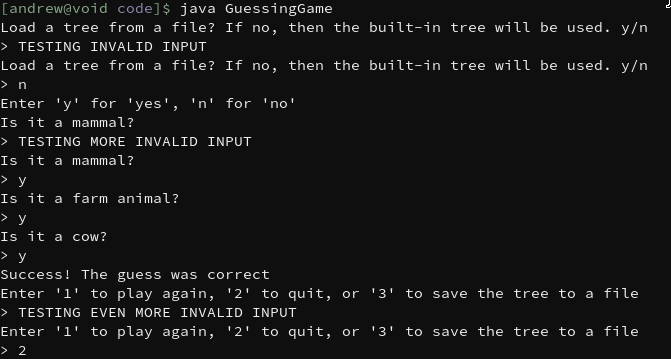
\includegraphics[width=0.7\textwidth]{./images/first.png}
    \caption{Basic Testing of the Game with the In-Built Tree}
\end{figure}

The next bit of testing is testing of an animal that the game doesn't know, adding it to the tree, and saving it to a file, as shown in the screenshot below.
\begin{figure}[h]
    \centering 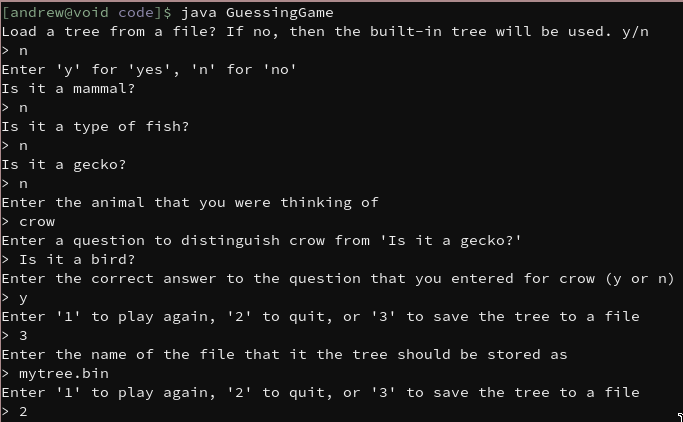
\includegraphics[width=0.7\textwidth]{./images/saving.png}
    \caption{Testing of the Saving a Tree to a File}
\end{figure}

\newpage
The next bit of testing is testing restoring a binary tree from a file on disk, using the file made above.
\begin{figure}[h]
    \centering 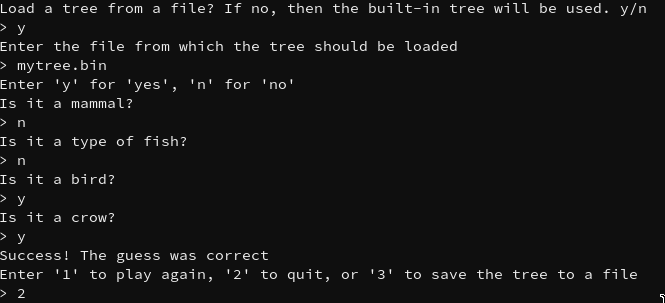
\includegraphics[width=0.7\textwidth]{./images/restore.png}
    \caption{Testing of the Restoring a Tree from a File}
\end{figure}

Testing trying to load a tree from a non-existent file on disk. This should loop until a valid input is given.
\begin{figure}[h]
    \centering 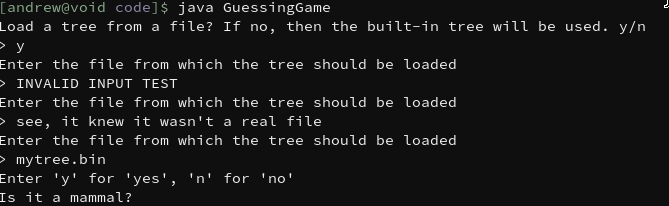
\includegraphics[width=0.7\textwidth]{./images/invalidtree.png}
    \caption{Testing Trying to Load a Non-Existent Tree File from Disk}
\end{figure}

Testing trying to load a normal text file as a binary tree file. 
Should throw an error and exit gracefully.
\begin{figure}[h]
    \centering 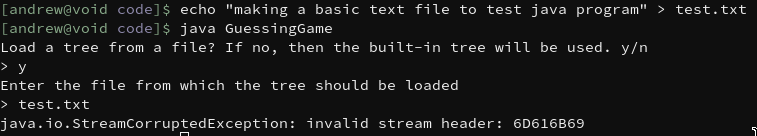
\includegraphics[width=0.7\textwidth]{./images/faketree.png}
    \caption{Testing Trying to Load a Non-Binary Tree File from Disk}
\end{figure}


\end{document}
